%-*-coding:utf-8;-*-
\documentclass[14pt]{beamer}
\usepackage[T1]{fontenc}
\usepackage[utf8]{inputenc}
%\usepackage[usenames,dvipsnames,svgnames,table]{xcolor}
\definecolor{links}{HTML}{2A1B81}
\hypersetup{colorlinks,linkcolor=,urlcolor=links}
\usetheme[numbering=none]{metropolis}           % Use metropolis theme
\setsansfont{Gentium}
\hyphenation{me-mo-ra-bi-li-um}
\title{Traces of Japan in Croatian Latin School Drama 1600–1800}
\date{29 June 2018}
\author{Nina Čengić, Neven Jovanović}
\institute{University of Zagreb, Faculty of Humanities and Social Sciences}
\begin{document}
  \maketitle
  


\begin{frame}
\tableofcontents
\end{frame}

\section{Croatia, Jesuits, and the Latin school drama}

{
    \usebackgroundtemplate{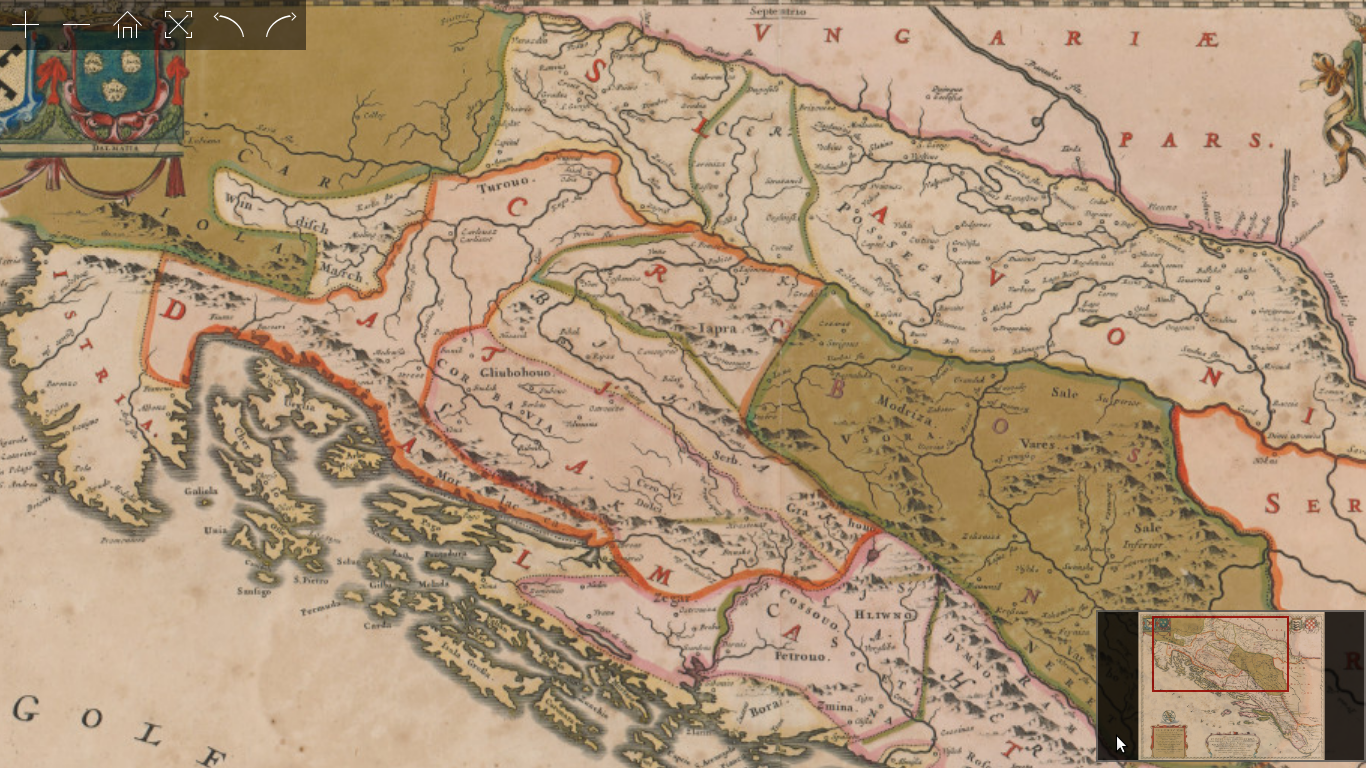
\includegraphics[width=\paperwidth]{img/illyricumhod.png}}
    \setbeamertemplate{navigation symbols}{}
    \begin{frame}[plain]
    \end{frame}
    }


\begin{frame}

Croatia (and Slavonia, and Dalmatia)

Kingdom of Hungary (and Croatia)

Habsburg Empire

Also: Republic of Venice, Republic of Dubrovnik (Ragusa)

\end{frame}


\begin{frame}{Jesuits in Croatia}

\alert{1559} Jesuit order comes to Dubrovnik

\alert{1604–1698} the Jesuits establish colleges in Dubrovnik, Zagreb, Rijeka, Varaždin, Požega

Jesuit colleges in Croatia were part of the Jesuit Austrian province.

\end{frame}

{
    \usebackgroundtemplate{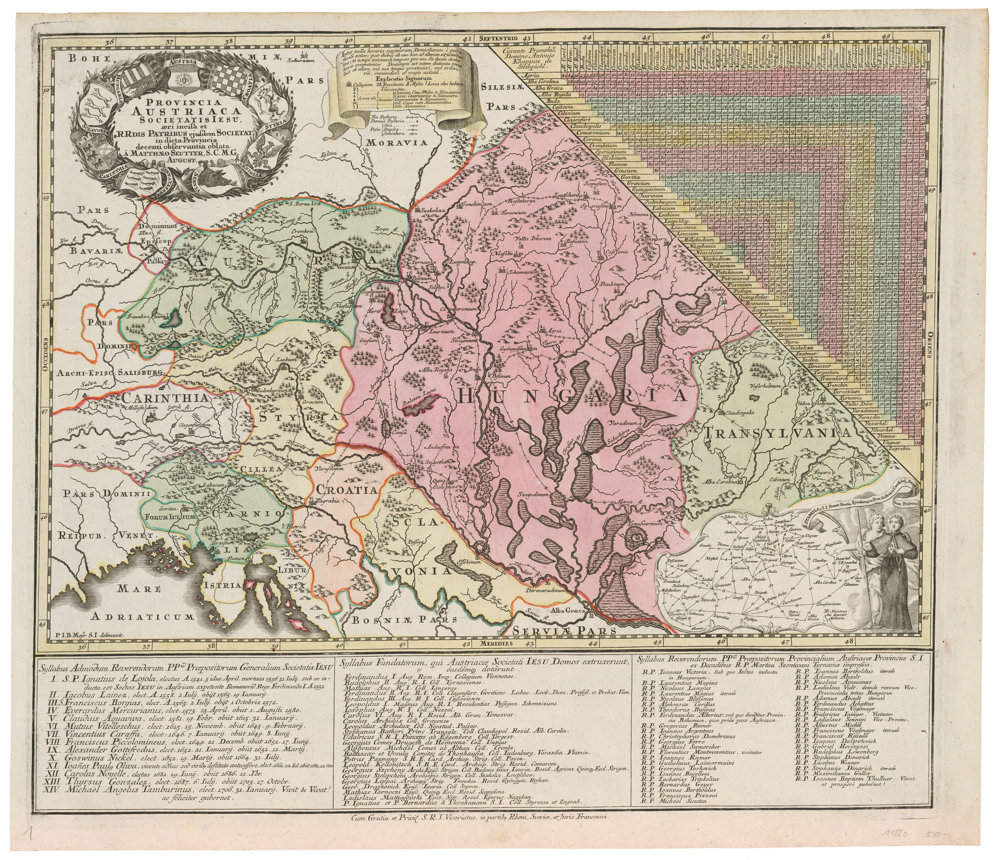
\includegraphics[width=\paperwidth]{img/eichler.jpeg}}
    \setbeamertemplate{navigation symbols}{}
    \begin{frame}[plain]
    \end{frame}
    }



\section{No research on Croatian Latin school drama until 2016?}


\begin{frame}[standout]

Not in the national language.

No texts, no authors.

Pedagogy, not original art.

Elitist and religious.

\end{frame}

\section{Sources}

\begin{frame}

Martina Petranović and Lucija Ljubić. \emph{Repertoar hrvatskih kazališta : Knjiga peta : Deskriptivna obrada važnijih predstava na hrvatskom jeziku i izvedbi na stranim jezicima hrvatskih izvođača do 1840. godine}, Zagreb 2012.

Staud, Géza. \emph{A magyarországi jezsuita iskolai színjátékok forrásai, III. : 1561-1773, Fontes ludorum scenicorum in scholis S. J. Hungariae, pars tertia}, Budapest 1988.

\end{frame}

\section{Methods}

\begin{frame}

An XML file holding records of performances.

An XML database with recorded searches.

A version-controlled repository with data, scripts, and documentation: \href{https://github.com/nevenjovanovic/croaladrama}{github.com/nevenjovanovic/croaladrama}.

The repository is freely available, can be updated, enhanced, integrated into larger collections.

\end{frame}

\section{Findings}

\begin{frame}{Findings}

The database holds records on \alert{686} performances in 1607–1805.

There are \alert{19} performances (2.6 percent) whose titles have to do with Japan.

\end{frame}

\begin{frame}{Findings}

The plays on Japan were performed during the 133 years between 1628 and 1761. 

They were performed in Jesuit colleges of the four cities:\\
\alert{Zagreb} (established 1606)\\
\alert{Varaždin} (Jesuits present from 1632, college established 1678)\\
\alert{Rijeka} (college established 1627)\\
\alert{Požega} (college established 1698).

\end{frame}

{
    \usebackgroundtemplate{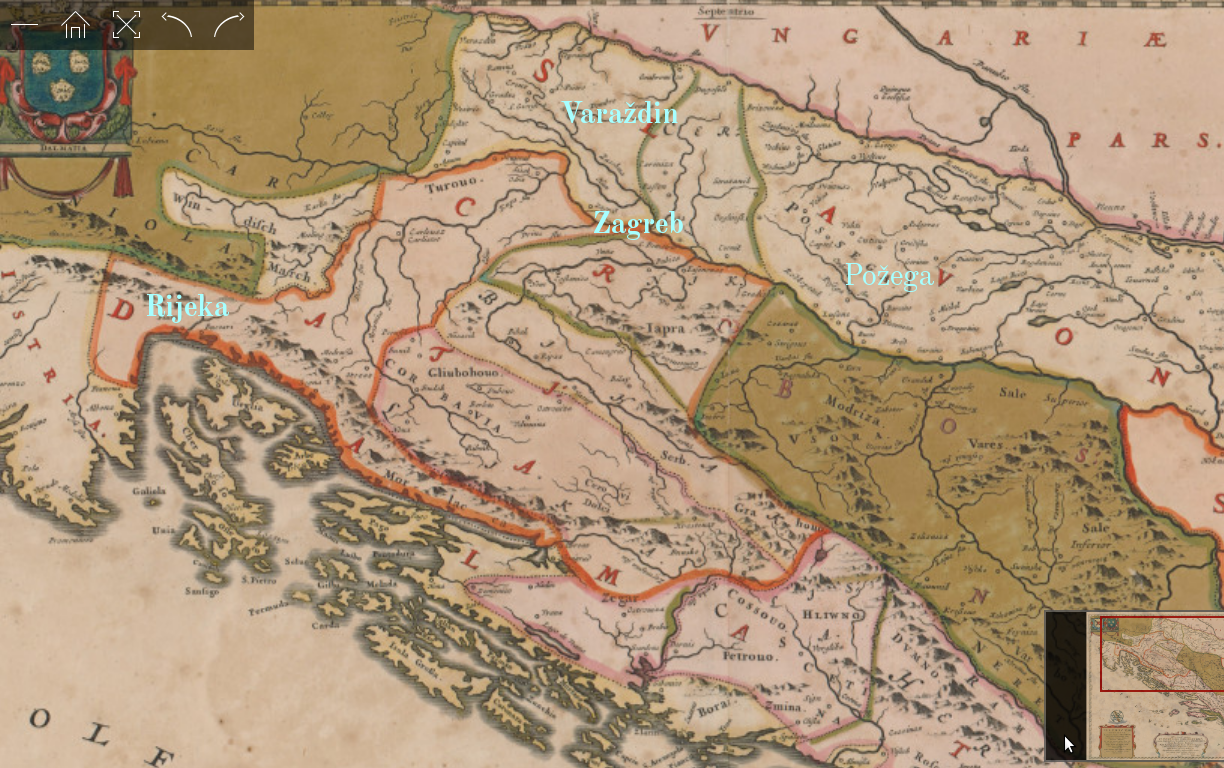
\includegraphics[width=\paperwidth]{img/illyricum_urb.png}}
    \setbeamertemplate{navigation symbols}{}
    \begin{frame}[plain]
    \end{frame}
    }

\begin{frame}{Findings}

Zagreb: \alert{six} performances 1628–1751\\
Varaždin: \alert{seven} performances 1713–1751\\
Rijeka: \alert{four} performances 1727–1747\\
Požega: \alert{two} performances 1735–1748

\end{frame}

\begin{frame}{An example: Performances in Rijeka}

\alert{1727} Triumphus fidei in quodam adolescente Japone\\
\alert{1735} Hero Christianus Japo\\
\alert{1740} Kimura e fuga ad fidem palamque martyrii revocatus\\
\alert{1747} Ucondus magnus

\end{frame}

\begin{frame}{A chronology}

\begin{enumerate}
\item \emph{Beginnings}: Zagreb 1628, 1677
\item \emph{The first wave}: Varaždin 1713; Zagreb 1716, 1720
\item Rijeka 1727
\item \emph{The second wave}: Varaždin 1733, 1734 (2); Rijeka 1735; Požega 1735; Varaždin 1737; Rijeka 1740
\item \emph{The third wave}: Varaždin 1744; Rijeka 1747; Požega 1748; Zagreb 1750; Varaždin 1751
\item \emph{Ending}: Zagreb 1761
\end{enumerate}

\end{frame}

\begin{frame}{Historical persons mentioned}

\begin{itemize}
\item Joannes Ingorus
\item Ludovicus Japoniae Martyr
\item Blessed father Luis Flores (19 August 1622)
\item Tokugawa Ieyasu (\href{http://www.wikidata.org/entity/Q171977}{www.wikidata.org/entity/Q171977})
\item Leonard Kimura (\href{http://www.wikidata.org/entity/Q11754482}{www.wikidata.org/entity/Q11754482}), Sebastian Kimura (\href{https://www.wikidata.org/entity/Q16185936}{www.wikidata.org/entity/Q16185936})
\end{itemize}

\end{frame}

\begin{frame}{Findings: testimonia from chronicles}

A spectacle


\end{frame}

\begin{frame}{A spectacle}

\alert{Zagreb 1628}: Diebus antecineralibus prodijt in theatrum Martyrium Joannis Ingori, filiorumque, in nouo orbe martyrium non ita pridem esse. Praemia.

\end{frame}

\begin{frame}{Findings: testimonia from chronicles}

Beautiful poetry


\end{frame}

\begin{frame}{Beautiful poetry}

\alert{Zagreb 1677}: Infima Japonicum adolescentem amoenissimis gratijs poëticis illustratum in scenam dedit.

\end{frame}

\begin{frame}{Findings: testimonia from chronicles}

Another spectacle


\end{frame}

\begin{frame}{Another spectacle}

\alert{Varaždin 1713}: Varasdini gloriatus uno de Ludovico Japoniae Martyre in quo Magistri, cujus nescio classis, industria nonnulla praemiola inter tubarum, tympanorumque fremitus. Praemia.

\end{frame}

\begin{frame}{Findings: testimonia from chronicles}

Good acting, well received


\end{frame}

\begin{frame}{Good acting}

\alert{Zagreb 1716}: Musae vero inferiores duabus potissimum actionibus dramaticis gloriantur, quarum alteram suprema et media classis grammatices exhibuit In triumpho crucis de Japone regulo et duobus filiis eius fortissimis fidei Christianae propugnatoribus. Tenuit illa mirifice spectatorum oculos ob vivacem adolescentum agendi modum in se defixos.

\end{frame}

\begin{frame}{Findings: testimonia from chronicles}

A model for the second-grade students

\end{frame}

\begin{frame}{A model for the second-grade students}

\alert{Zagreb 1720}: Principistae exhibuerunt Phirandum Japonem Christianum principistam fidei rudimenta sangvine et vita defendere paratum.

\end{frame}

\section{Conclusions}

\begin{frame}{Conclusions}

The Jesuit school theatre offered to virtually all Croatian intellectuals during the 17th and 18th century a chance to perform in front of an audience. 

Theatre and performance were an integral part of the education.

Being on stage was an early experience of each Croatian intellectual.


\end{frame}

\begin{frame}{Conclusions}

The thematic range of the Jesuit school theatre was not limited to one's own country and one's own nation. 

The Jesuit interest for Japan suggests an interest for modernity, even when expressed in the language of Cicero and Saint Jerome. 




\end{frame}

\begin{frame}{Conclusions}

The presence, and nurture, of such modern interests in a small Slavic community at the periphery of the Habsburg Empire means that the horizons were wider than we are ready to admit today.

\end{frame}



  \maketitle


\end{document}
Lucretius 
